\section{Exploratory Perturbation Scenarios}

The separated exploratory module uses restrained perturbation scenarios involving morphology, HCN, potassium, AMPA/NMDA, clustering, synchrony, combined perturbations, and conflicting directions \citep{Bender2003HCN,Kole2007HCN1Loss,Nava2014HCN1,Losonczy2008CompartmentalizedPlasticity,Jarsky2005DendriticSpikePropagation}. The source rows explicitly mark these scenarios as exploratory-only and make no diagnostic or therapeutic claim.

The exploratory uncertainty screen uses N=8 sampled combinations per scenario. It is a sensitivity screen rather than a biological uncertainty estimate or rare-tail analysis. The exploratory scenarios are best cited as examples showing that synaptic strength, active state, clustering, and timing can alter voltage outcomes without changing morphology-defined SMI.

\begin{figure}[!htbp]
\centering
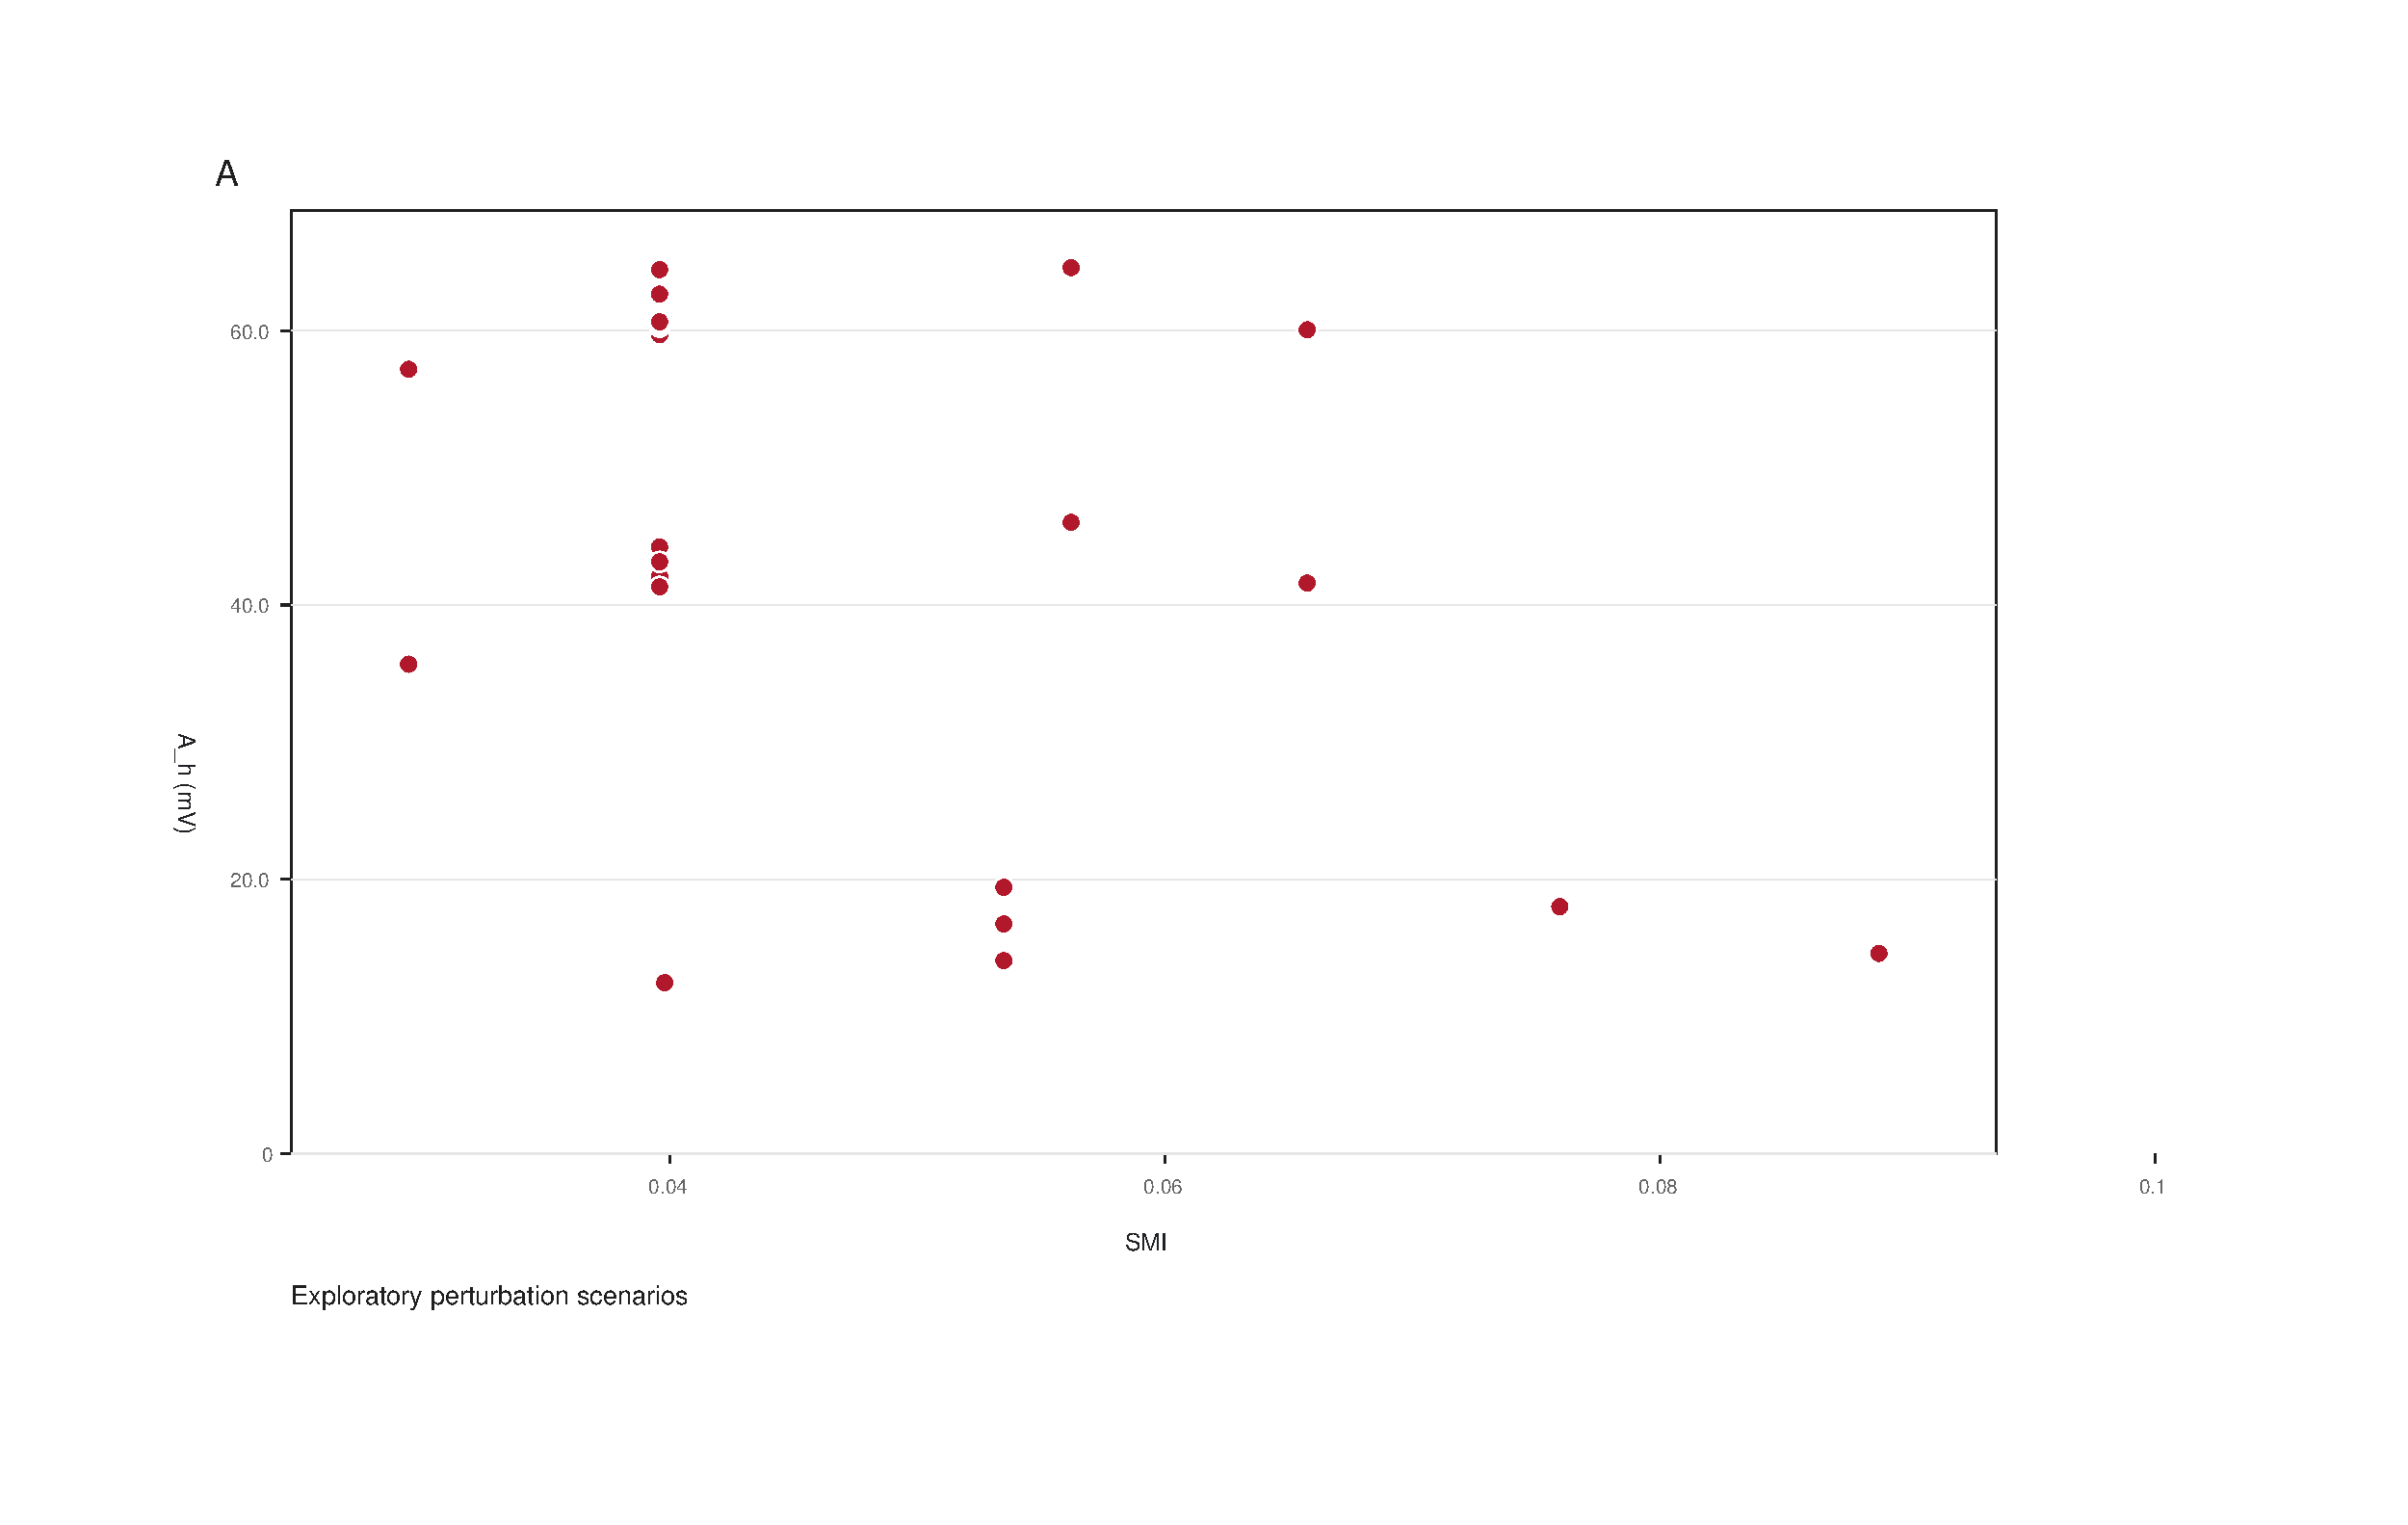
\includegraphics[width=0.85\textwidth,keepaspectratio]{../figures_publication/FigS8_phase06_smi_amplitude.pdf}
\caption{\textbf{Figure S8.} Exploratory perturbation scenarios showing SMI versus head amplitude. These cases remain separated from the general model and are not used to support primary claims.}
\label{fig:s8_phase06_amplitude}
\end{figure}

\begin{figure}[!htbp]
\centering
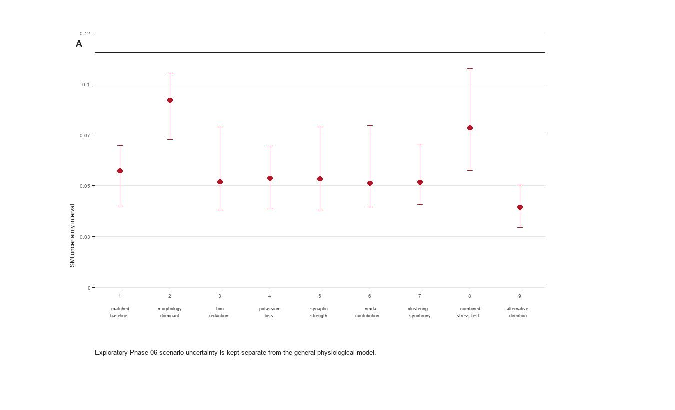
\includegraphics[width=0.85\textwidth,keepaspectratio]{../figures_publication/FigS9_phase06_uncertainty.pdf}
\caption{\textbf{Figure S9.} Scenario-level SMI uncertainty screen. Intervals summarize exploratory perturbation scenarios and are presented as context rather than primary validation evidence.}
\label{fig:s9_phase06_uncertainty}
\end{figure}
